<<<<<<< HEAD
\chapter{Mengenal Kecerdasan Buatan dan Scikit-Learn}
Buku umum yang digunakan adalah \cite{russell2016artificial} dan
untuk sebelum UTS menggunakan buku \textit{Python Artificial Intelligence Projects for Beginners}\cite{eckroth2018python}.
Dengan praktek menggunakan python 3 dan editor anaconda dan library python scikit-learn.
Tujuan pembelajaran pada pertemuan pertama antara lain:
\begin{enumerate}
\item
Mengerti definisi kecerdasan buatan, sejarah kecerdasan buatan, perkembangan dan penggunaan di perusahaan
\item
Memahami cara instalasi dan pemakaian sci-kit learn
\item
Memahami cara penggunaan variabel explorer di spyder
\end{enumerate}
Tugas dengan cara dikumpulkan dengan pull request ke github dengan menggunakan latex pada repo yang dibuat oleh asisten riset.

\section{Teori}
Praktek teori penunjang yang dikerjakan :
\begin{enumerate}
\item
Buat Resume Definisi, Sejarah dan perkembangan Kecerdasan Buatan, dengan bahasa yang mudah dipahami dan dimengerti. Buatan sendiri bebas plagiat[hari ke 1](10)
\item
Buat Resume mengenai definisi supervised learning, klasifikasi, regresi dan unsupervised learning. Data set, training set dan testing set.[hari ke 1](10)
\end{enumerate}

\section{Instalasi}
Membuka https://scikit-learn.org/stable/tutorial/basic/tutorial.html. Dengan menggunakan bahasa yang mudah dimengerti dan bebas plagiat.
Dan wajib skrinsut dari komputer sendiri.
\begin{enumerate}
\item
Instalasi library scikit dari anaconda, mencoba kompilasi dan uji coba ambil contoh kode dan lihat variabel explorer[hari ke 1](10)
\item
Mencoba Loading an example dataset, menjelaskan maksud dari tulisan tersebut dan mengartikan per baris[hari ke 1](10)
\item
Mencoba Learning and predicting, menjelaskan maksud dari tulisan tersebut dan mengartikan per baris[hari ke 2](10)
\item
mencoba Model persistence, menjelaskan maksud dari tulisan tersebut dan mengartikan per baris[hari ke 2](10)
\item
Mencoba Conventions, menjelaskan maksud dari tulisan tersebut dan mengartikan per baris[hari ke 2](10)
\end{enumerate}


\section{Penanganan Error}
Dari percobaan yang dilakukan di atas, apabila mendapatkan error maka:

\begin{enumerate}
	\item
	skrinsut error[hari ke 2](10)
	\item
Tuliskan kode eror dan jenis errornya [hari ke 2](10)
	\item
Solusi pemecahan masalah error tersebut[hari ke 2](10)

\end{enumerate}

\section{Teori/Fadila/1164072}
Teori mencakup resume dari beberapa pembahasan. yaitu :
\begin{enumerate}
\item Tentang Kecerdasan Buatan
\begin{itemize}
\item Definisi Kecerdasan Buatan.
\par Kecerdasan Buatan biasa disebut dengan istilah AI ( Artificial Intelligence ) . AI sendiri merupakan suatu cabang dalam bidang sains komputer sains dimana mengkaji tentang bagaimana cara untuk melengkapi sebuah komputer dengan kemampuan atau kepintaran layaknya atau mirip dengan yang dimiliki manusia. Sebagai contoh, sebagaimana komputer dapat berkomunikasi dengan pengguna baik menggunakan kata, suara maupun lain sebagainya . Dengan kemampuan ini, diharapkan komputer mampu mengambil keputusan sendiri untuk berbagai kasus yang ditemuinya kemudian itulah yang disebut dengan kecerdasan buatan.
\par  Kecerdasan buatan makin canggih dengan kemampuan komputer dalam memperbarui pengetahuannya dengan banyaknya testing dan perkembangan target analisa. Untuk kecerdasan buatan ada banyak contoh dan jenisnya. Salah satu contoh yang paling terkenal dari Artificial Intelligence ialah Google Assistant. Google Assistant digunakan untuk kemudahan user dalam menemukan berbagai hal maupun penyettingan langsung terhadap smartphone yang digunakan dan masih banyak lagi.
\item Sejarah Kecerdasan Buatan
\par Artificial intelligence merupakan inovasi baru di bidang ilmu pengetahuan. Mulai terbentuk sejak adanya komputer modern dan kira-kira terjadi sekitaran tahun 1940 dan 1950. Ilmu pengetahuan komputer ini khusus ditujukan dalam perancangan otomatisasi tingkah laku cerdas dalam sistem kecerdasan komputer.
\par Pada awalnya, kecerdasan buatan hanya ada di universitas-universitas dan laboratorium penelitian, serta hanya sedikit produk yang dihasilkan dan dikembangkan. Menjelang akhir 1970-an dan 1980-an, mulai dikembangkan secara penuh dan hasilnya berangsur-angsur dipublikasikan di khalayak umum.
\par

\begin{figure}[ht]
\centering
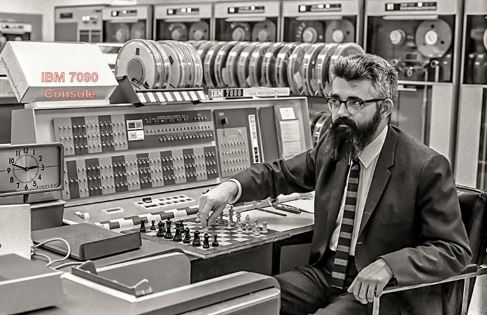
\includegraphics[scale=0.5]{figures/contoh.jpg}
\caption{capturing}
\label{contoh}
\end{figure}

\par Jika kita berbicara tentang AI atau Artificial Intelligence maka kita tidak bisa melupakan seorang sosok yang sangat terkenal pada bidang tersebut yaitu bapak John McCarthy.
McCarthy mendapatkan gelar sarjana matematika dari California Institute of Technology (Caltech) pada September 1948. Dari masa kuliahnya itulah ia mulai mengembangkan ketertarikannya pada mesin yang dapat menirukan cara berpikir manusia. McCarthy kemudian melanjutkan pendidikan ke program doktoral di Princeton University.

\par McCarthy kemudian mendirikan dua lembaga penelitian kecerdasan buatan. Kedua lembaga AI itu adalah Stanford Artificial Intelligence Laboratory dan MIT Artificial Inteligence Laboratory. Di lembaga-lembaga inilah bermunculan inovasi pengembangan AI yang meliputi bidang human skill, vision, listening, reasoning dan movement of limbs. Bahkan Salah satu lembaga yang didirikan itu, Stanford Artificial Intelligence pernah mendapat bantuan dana dari Pentagon untuk membuat teknologi-teknologi luar angkasa.

\item Perkembangan Kecerdasan Buatan
\par Teknologi Artificial Intelligence semakin ramai dibahas dalam berbagai diskusi teknologi di seluruh dunia.Menurut kebanyakan orang, pekerjaan seperti kasir, operator telepon, pengendara truk, dan lainnya sangat berpeluang besar untuk tergantikan oleh Artificial Intelligence. Mengapa terjadi hal demikian? dikarenakan memang bahwa AI lebih ungul dalam hal kinerja, fitur dan lain sebagainya. Namun, dalam beberapa aspek memang pekerja manusia masih unggul dibandingkan AI itu sendiri.
\par Para generasi muda yang ada di dunia terutama di daerah Asia terlihat sudah memahami fungsi dan efek dari AI dalam kehidupan kita sehari-hari. Berdasarkan survei yang dilakukan oleh Microsoft, terdapat 39 persen responden yang mempertimbangkan untuk menggunakan mobil tanpa pengemudi dan 36 persen lainnya setuju bahwa robot masa depan dengan software untuk beroperasi mampu meningkatkan produktivitas. Dari survey tersebut kita sebagai pengguna AI harus lebih bijaksana dalam pengembangan dan penggunaan dari AI sehingga tanpa memberikan efek samping terhadap etos kerja dan keseharian kita sebagai pengguna dalam kehidupan sehari-hari.
\end{itemize}
\item Tentang Pengertian Terhadap Ilmu Yang Lain
\begin{itemize}
\item Supervised Learning adalah pendekatan dimana sudah terdapat data yang dilatih selain itu juga terdapat variable yang ditargetkan sehingga tujuan dari pendekatan ini yaitu mengkelompokan suatu data ke data yang sudah ada.
\par
\item Klasifikasi adalah pembagian sesuatu menurut kelas-kelas ( class ). Menurut Ilmu Pengetahuan, Klasifikasi merupakan proses pengelompokkan benda berdasarkan ciri-ciri persamaan dan juga perbedaan.
\par
\item Regresi adalah metode analisis statistik yang digunakan untuk melihat pengaruh antara dua ataupun lebih variabel.
\par
\item Unsupervised Learning berbeda dengan Supervised Leraning. Perbedaannya ialah unsupervised learning tidak memiliki data latih, sehingga dari data yang ada kita mengelompokan data tersebut menjadi 2  ataupun 3 bagian dan seterusnya.
\par
\item Dataset adalah objek yang merepresentasikan data dan juga relasi yang ada di memory. Strukturnya mirip dengan data di database, namun bedanya dataset berisi koleksi dari data table dan data relation.
\par
\item Training Set adalah set digunakan oleh algoritma klassifikasi . Dapat dicontohkan dengan :  decision tree, bayesian, neural network dll. Semuanya dapat digunakan untuk membentuk sebuah model classifier.
\par
\item Testing Set adalah set yang digunakan untuk mengukur sejauh mana classifier berhasil melakukan klasifikasi dengan benar.
\par
\end{itemize}
\end{enumerate}


\section{Instalasi/Fadila/1164072)}
Untuk Instalasinya mencakup i beberapa pembahasan dan tutorial. yaitu :
\begin{enumerate}
\item Instalasi Scikit-Learn Dari Anaconda
\begin{itemize}
\item Instalasi Anaconda
\begin{enumerate}
\item Pertama-tama silahkan pastikan bahwa anda telah melakukan instalasi software Anaconda.
\item Apabila belum, silahkan buka web browser anda untuk melakukan pengunduhan software Anaconda
\item Setelah terunduh, silahkan klik kanan lalu run administrator pada software Anaconda
\item Silahkan lakukan penginstalan dengan menekan tombol install pada tampilan instalasi
\item Kemudian tekan tombol next maka akan sampai pada tampilan diatas

\par

\begin{figure}[ht]
\centering
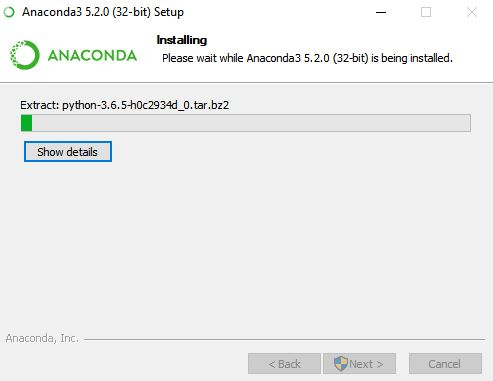
\includegraphics[scale=0.5]{figures/ana1.jpg}
\caption{install anaconda 1}
\label{contoh}
\end{figure}

\par
\item Selanjutnya apabila instalan tersebut telah selesai maka silahkan menekan tombol next
\item Tampilan selanjutnya akan seperti ini

\par

\begin{figure}[ht]
\centering
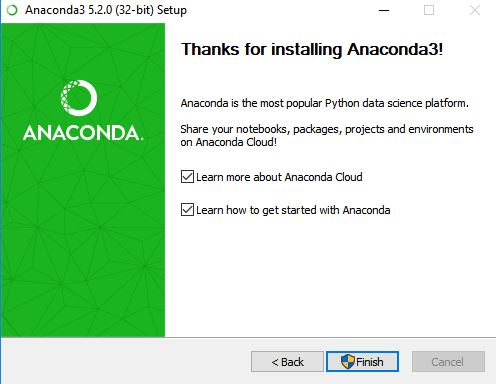
\includegraphics[scale=0.5]{figures/ana2.jpg}
\caption{install anaconda 2}
\label{contoh}
\end{figure}

\par

\item Apabila tampilannya telah sesuai dengan contoh gambar maka instalasi telah selesai
\end{enumerate}
\end{itemize}

\begin{itemize}
\item Instalasi Library Scikit Learn
\begin{enumerate}
\item Silahkan membuka web browser untuk melakukan pengunduhan untuk library scikit dari anaconda.
\item Silahkan mengunjungi halaman ini untuk melakukan pengunduhan library scikit dari anaconda.
\par https://anaconda.org/anaconda/scikit-learn.
\item Setelah terdownload silahkan melakukan instalasi lanjutan menggunakan Command Prompt
\item Silahkan masukkan perintah berikut untuk melakukan pengecekan bahwa anaconda anda telah terpasang dengan baik.
\par conda --version
\par python --version
\item Tampilannya akan nampak seperti berikut :
\par

\begin{figure}[ht]
\centering
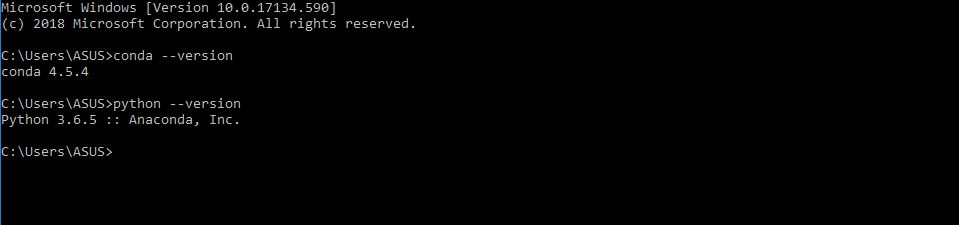
\includegraphics[scale=0.3]{figures/scikit1.jpg}
\caption{Pengecekan Anaconda}
\label{contoh}
\end{figure}

\par
\item Selanjutnya silahkan masukkan perintah berikut untuk melakukan instalasi pip sckit-learn
\par perintahnya : pip install -U scikit-learn
\item Tampilannya akan nampak seperti berikut :
\par

\begin{figure}[ht]
\centering
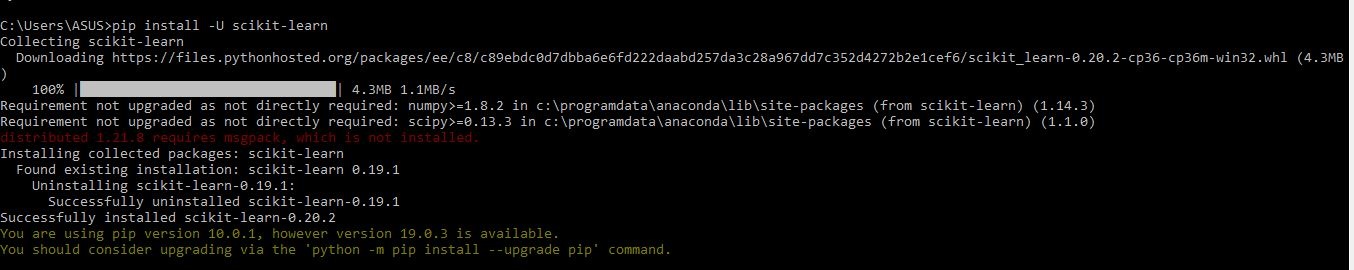
\includegraphics[scale=0.2]{figures/scikit3.jpg}
\caption{instalasi pip scikit-learn}
\label{contoh}
\end{figure}

\par
\item Selanjutnya silahkan masukkan perintah berikut untuk melakukan instalasi conda sckit-learn
\par perintahnya : conda install scikit-learn
\item Tampilannya akan nampak seperti berikut :
\par

\begin{figure}[ht]
\centering
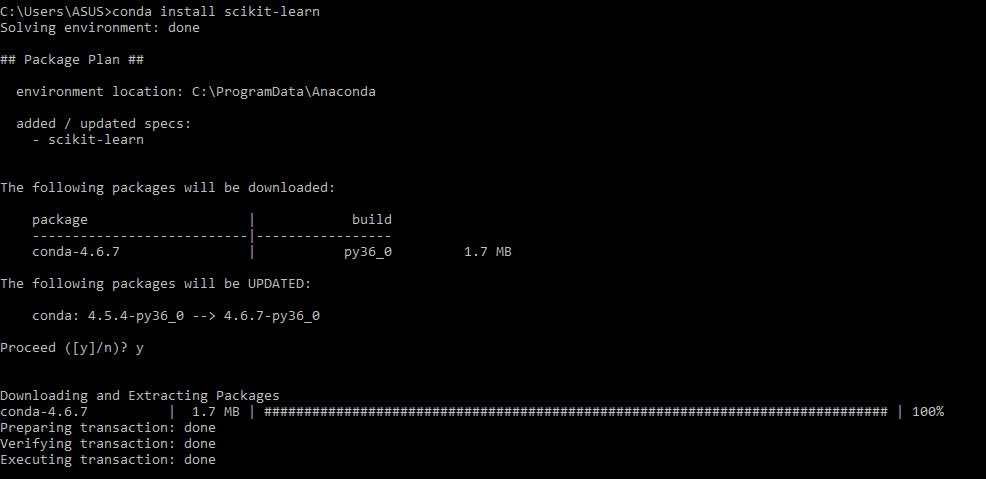
\includegraphics[scale=0.3]{figures/scikit4.jpg}
\caption{instalasi conda scikit-learn}
\label{contoh}
\end{figure}

\par
\par
\par
\item Apabila telah dipraktekan seperti langkah-langkah dan menghasilkan tampilan seperti contoh diatas, maka instalasi scikit-learn dari anaconda berhasil dilakukan
\par
\item Kemudian untuk pengujian yang lain yaitu pengujian untuk mengecek codingan anaconda
\par
\item Contoh uji coba codingannya dapat dilihat pada gambar berikut
\par
\begin{figure}[ht]
\centering
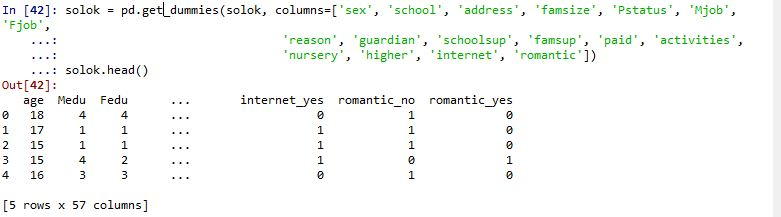
\includegraphics[scale=0.5]{figures/3.jpg}
\caption{uji coba codingan}
\label{contoh}
\end{figure}
\par
\item Berdasarkan pengujian tersebut maka dapat dipastikan bahwa anaconda telah ter-include ke dalam python dan dieksekusi dengan script python
\item Setelah pengeksekusiannya berdasarkan scripts python, terdapatlah keluaran yang sesuai
\item Keluaran tersebut yang menandakan bahwa anacondanya berfungsi dengan baik.
\end{enumerate}
\end{itemize}


\par
\item Loading An Example Dataset
\begin{itemize}
\item Penerapan Loading An Example Dataset Pada Python Di CMD
\begin{enumerate}
\item Pertama-tama silahkan buka command prompt di laptop anda
\item Selanjutnya masuk ke python
\item Setelah masuk kedalam python, silahkan masukkan perintah seperti pada gambar berikut :

\begin{figure}[ht]
\centering
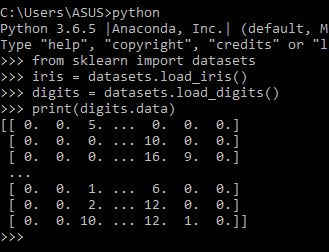
\includegraphics[scale=0.6]{figures/4.jpg}
\caption{pengujian loading an example dataset}
\label{contoh}
\end{figure}

\par
\item Secara keseluruhan, hasilnya pada command prompt akan nampak seperti gambar tersebut
\item Apabila tampilanya telah nampak seperti gambar diatas, maka pengujiannya telah selesai dan berhasil.
\end{enumerate}

\par
\item Penjelasan Perintah Yang Di Uji
\begin{enumerate}
\item Perhatikan perintah yang telah dieksekusi ini :

\par
\begin{figure}[ht]
\centering
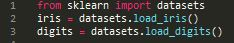
\includegraphics[scale=0.9]{figures/ok4.jpg}
\caption{pengujian loading an example dataset}
\label{contoh}
\end{figure}
\par

\item Penjelasan untuk baris pertama ialah :
\par Perintahnya yaitu memasukkan dan memanggil dataset dari sklearn
\par
\par
\item Penjelasan untuk baris kedua ialah :
\par Terdapat variabel baru yaitu iris. Dimana variabel iris memanggil datasets dan di dalamnya akan ngeload ( menampilkan ) load iris.
\par
\item Penjelasan untuk baris ketiga ialah :
\par Kemudian ada juga variabel baru lainnya yaitu digits yang akan memanggil dataset dan di dalamnya akan ngeload ( menampilkan ) load digits
\par
\item Selanjutnya untuk perintah Print( digits.data ) ditujukan untuk me-
\par nampilkan output dari pengeksekusian variabel digits dan akan berupa data.
\par
\item Hasilnya printnya sebagai berikut :
\par

\begin{figure}[ht]
\centering
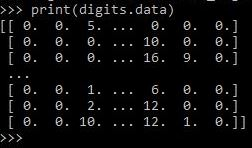
\includegraphics[scale=0.7]{figures/okk4.jpg}
\caption{hasil print uji cobat}
\label{contoh}
\end{figure}

\par
\item Untuk penjelasan uji cobanya sudah selesai.
\par
\end{enumerate}
\end{itemize}
\end{enumerate}

\section{Teori/Rahmi Roza/1164085}
Teori mencakup resume dari beberapa pembahasan. yaitu :
\begin{itemize}
\item Definisi Kecerdasan Buatan.
\par Kecerdasan Buatan adalah salah satu cabang Ilmu pengetahuan berhubungan dengan pemanfaatan mesin untuk memecahkan persoalan yang rumit dengan cara yang lebih manusiawi. Hal Ini biasanya dilakukan dengan mengikuti/mencontoh karakteristik dan analogi berpikir dari kecerdasan/Inteligensia manusia, dan menerapkannya sebagai algoritma yang dikenal oleh komputer.
\par Agar komputer bisa bertindak seperti dan sebaik manusia, maka komputer juga harus diberi bekal pengetahuan dan mempunyai kemampuan untuk menalar. Untuk itu AI akan mencoba untuk memberikan beberapa metoda untuk membekali komputer dengan kedua komponen tersebut agar komputer bisa menjadi mesin pintar.
\item Sejarah Kecerdasan Buatan
\par Banyak orang percaya kecerdasan buatan akan memusnahkan kelangsungan hidup manusia saat mereka menyadari kekuatan yang dimilikinya. Semua bermula sejak Turing Machine. Berikut perjalanan kecerdasan buatan hingga akhirnya melahirkan robot dan robot seks.
\par Tahun 1950. Alan Turing memperkenalkan Turing Test dalam jurnal berjudul Computering Machinery and Intelligence. Pada musim panas 1956, Konferensi Dartmouth meluncurkan ide artificial intelligence dan IBM memulai riset tentang AI.
\par Tahun 1970. Sepanjang 1974 sampai 1980 merupakan gelombang pertama kecerdasan buatan. Pada periode ini pula pengumpulan dana untuk melakukan riset kecerdasan buatan mulai marak.
\par Tahun 1930. Pada 11 Mei 1997, Deep Blue Computer, kecerdasan buatan besutan IBM berhasil mengalahkan grand master catur asal Rusia, Garry Kasparov
\par Tahun 2000. Kendaraan bikinan tim peneliti dari Universitas Stanford, Amerika Serikat, berhasil menjadi kampiun dal DARPA Grand Challange. Mobil swakemudi ini bisa melaju di gurun pasir sejauh 211 kilometer.
\par Tahun 2010. Watson, kecerdasan buatan besutan IBM, berhasil mengalahkan mantan juara Brad Rutter dan Ken Jennings dalam acara kuis Jeopardy pada pertengahan 2011. Appel, pada 14 Oktober tahun yang sama, memperkenalkan asistem pribadi berbasiskan kecerdasan buatan bernama Siri dalam iPhone 4s. Setahun kemudian, tepatnya Juni, tim dari Google Brain melatih komputer agar bisa mengenali seekor kucing dari jutaan video di YouTube.ChatBot bikinin Eugene Goostman mengklaim telah memecahkan tes Turing dalam kompetisi yang digelar di Universitas Reading, Inggris. Imbasnya, pada Agustus tahun yang sama, banyak ilmuwan mengusulkan untuk membuat tes Turing yang baru. Sementara itu, terkesan dengan kemampuan Watson, NASA menggunakannya untuk penelitian bidang kedirgantaraan.
\par Tahun 2017. Google, Februari lalu, kembali membuat gebrakan soal kecerdasan buatan. Tim dari Google Deep Mind mengungkap kecerdasan buatan memiliki tingkat emosi dan kemarahan yang sama dengan manusia. Kecerdasan buatan pun bisa merasakan kalau dirinya ditipu. Tak mau kalah, Microsoft, April lalu, mendeteksi bahwa artificial intelligence ternyata juga bisa rasis.
Yang paling fenomenal soal kecerdasan buatan pada tahun ini adalah robot seks bernama Harmony. Tak seperti robot seks pada umumnya, Harmony bisa merasakan cemburu dan mendeteksi penggunanya saat hendak menuju klimaks.
\par Jika kita berbicara tentang AI atau Artificial Intelligence maka kita tidak bisa melupakan seorang sosok yang sangat terkenal pada bidang tersebut yaitu bapak John McCarthy.
McCarthy mendapatkan gelar sarjana matematika dari California Institute of Technology (Caltech) pada September 1948. Dari masa kuliahnya itulah ia mulai mengembangkan ketertarikannya pada mesin yang dapat menirukan cara berpikir manusia. McCarthy kemudian melanjutkan pendidikan ke program doktoral di Princeton University.
\par McCarthy kemudian mendirikan dua lembaga penelitian kecerdasan buatan. Kedua lembaga AI itu adalah Stanford Artificial Intelligence Laboratory dan MIT Artificial Inteligence Laboratory. Di lembaga-lembaga inilah bermunculan inovasi pengembangan AI yang meliputi bidang human skill, vision, listening, reasoning dan movement of limbs. Bahkan Salah satu lembaga yang didirikan itu, Stanford Artificial Intelligence pernah mendapat bantuan dana dari Pentagon untuk membuat teknologi-teknologi luar angkasa.

\item Perkembangan Kecerdasan Buatan
\par Perkembangan kecerdasan buatan atau artificial intelligence (AI) dinilai tidak bisa dihentikan. Keberadaan AI justru dinilai akan semakin mempermudah kehidupan manusia dalam beraktivitas. Dalam pandangan Johnny Lie sebagai Vice President of Cheetah Mobile, revolusi teknologi tidak bisa dihentikan. Menurutnya, hal itu sudah terjadi sejak puluhan tahun yang lalu. Cheetah Mobile sendiri merupakan perusahaan teknologi mobile yang fokus pada peranti lunak dan pada hari ini menyematkan unsur AI dalam layanannya.
\par Sebelumnya, beberapa pakar teknologi kenamaan dunia, seperti Elon Musk dan Stephen Hawking gencar memberikan peringatan bahwa AI yamg terus berkembang dapat menjadi ancaman bagi umat manusia. Bahkan, keduanya bersama banyak ilmuwan lainnya membuat surat penegasan kepada PBB untuk mengawasi pertumbuhan AI.
\par Dengan AI, sebuah produk teknologi dapat bekerja lebih cerdas dan mandiri. Misalnya saja, sebuah aplikasi smartphone yang menggunakan AI dapat mempelajari kebiasaan pengguna. Alhasil, Anda tidak perlu repot lagi dalam melakukan suatu pekerjaan di ponsel.
\end{itemize}
\item Tentang Pengertian Terhadap Ilmu Yang Lain
\begin{itemize}
\item Supervised learning adalah sebuah pendekatan dimana sudah terdapat data yang dilatih, dan terdapat variable yang ditargetkan sehingga tujuan dari pendekatan ini adalah mengkelompokan suatu data ke data yang sudah ada
\par
\item Klasifikasi adalah pembagian sesuatu menurut kelas-kelas ( class ). Menurut Ilmu Pengetahuan, Klasifikasi merupakan proses pengelompokkan benda berdasarkan ciri-ciri persamaan dan juga perbedaan.
\par
\item Regresi adalah metode analisis statistik yang digunakan untuk melihat pengaruh antara dua ataupun lebih variabel.
\par
\item Unsupervised Learning berbeda dengan Supervised Leraning. Perbedaannya ialah unsupervised learning tidak memiliki data latih, sehingga dari data yang ada kita mengelompokan data tersebut menjadi 2  ataupun 3 bagian dan seterusnya.
\par
\item Dataset adalah objek yang merepresentasikan data dan juga relasi yang ada di memory.
\par
\item Training Set adalah set digunakan oleh algoritma klassifikasi . Dapat dicontohkan dengan :  decision tree, bayesian, neural network dll. Semuanya dapat digunakan untuk membentuk sebuah model classifier.
\par
\item Testing Set adalah set yang digunakan untuk mengukur sejauh mana classifier berhasil melakukan klasifikasi dengan benar.
\par
\end{itemize}
\end{enumerate}

\section{Instalasi/Rahmi Roza/1164085}
\begin{figure}[ht]
\centering
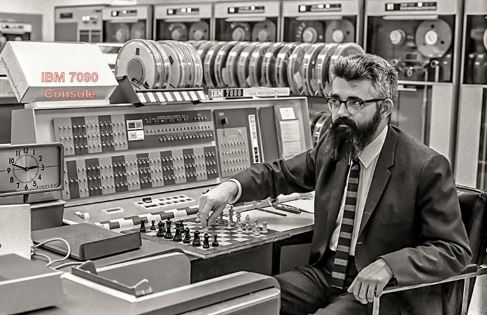
\includegraphics[scale=0.5]{figures/contoh.jpg}
\caption{gambar1}
\label{roza1}
\end{figure}

\begin {enumerate}
\item Baris 1 = memasukkan dan memanggil svm dari sklearn
\item Baris 2 = membuat variable
\end {enumerate}

\begin{figure}[ht]
\centering
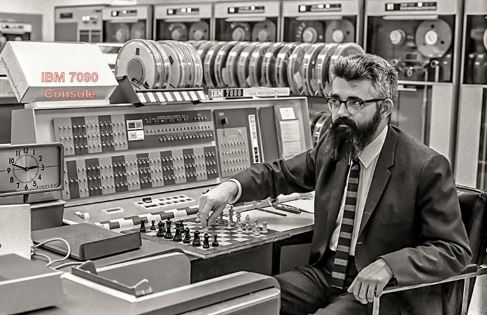
\includegraphics[scale=0.7]{figures/contoh.jpg}
\caption{gambar2}
\label{roza2}
\end{figure}

\begin {enumerate}
\item Baris 1 = clf dipasang pada model fit metode
\item Baris 2 =  implementasikan klasifikasi dukungan vektor
\end {enumerate}

\begin{figure}[ht]
\centering
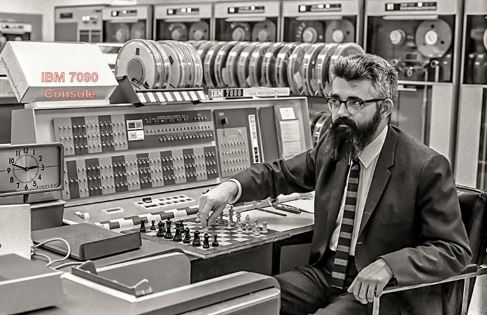
\includegraphics[scale=0.5]{figures/contoh.jpg}
\caption{gambar3}
\label{roza3}
\end{figure}

\begin {enumerate}
\item Baris 1 = prediksi nilai baru
\item Baris 2 = set array
\end {enumerate}

\begin{figure}[ht]
\centering
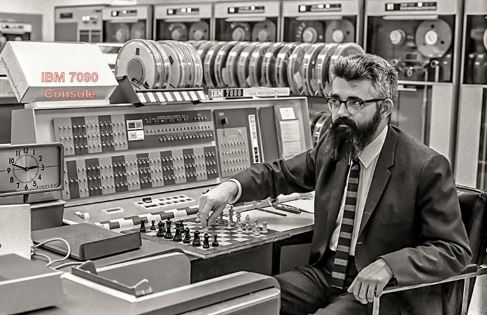
\includegraphics[scale=0.10]{figures/contoh.jpg}
\caption{gambar4}
\label{roza4}
\end{figure}

\begin {enumerate}
\item Baris 1 = memasukkan dan memanggil datasets dari sklearn
\item Baris 2 = memasukkan dan memanggil svm dari sklearn
\item Baris 3 = membuat variable clf
\item Baris 4 = membuat variable iris
\item Baris 5 = membuat variable x, y
\item Baris 6 = clf dipasang pada model fit metode
\item Baris 7 = implementasikan klasifikasi dukungan vektor
\item Baris 8 = memanggil library pickle
\item Baris 9 = membuat variable s
\item Baris 10 = membuat variable clf2
\item Baris 11 = prediksi nilai baru
\item Baris 12 = set array
\end {enumerate}

\begin{figure}[ht]
\centering
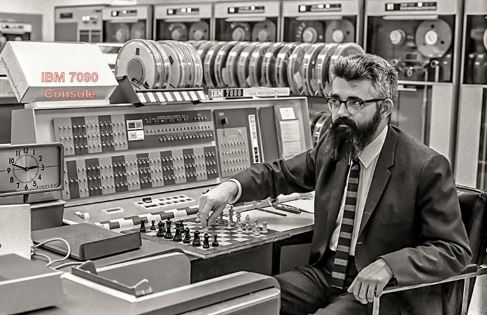
\includegraphics[scale=0.7]{figures/contoh.jpg}
\caption{gambar5}
\label{roza5}
\end{figure}

\begin {enumerate}
\item Baris 1 = memasukkan dan memanggil numpy sebagai np
\item Baris 2 = memasukkan dan memanggil random_projection dari sklearn
\item Baris 3 = membuat variable rng
\item Baris 4 = membuat variable rng
\item Baris 5 = membuat variable x
\item Baris 6 = pemanggilan variable x
\item Baris 7 = pemanggilan dtype
\item Baris 8 = membuat variable tranformer
\item Baris 9 = membuat variable x_new
\item Baris 10 = pemanggilan x_new
\item Baris 11 = pemanggilan dtype
\end {enumerate}

\chapter{Mengenal Kecerdasan Buatan dan Scikit-Learn}
Buku umum yang digunakan adalah \cite{russell2016artificial} dan
untuk sebelum UTS menggunakan buku \textit{Python Artificial Intelligence Projects for Beginners}\cite{eckroth2018python}.
Dengan praktek menggunakan python 3 dan editor anaconda dan library python scikit-learn.
Tujuan pembelajaran pada pertemuan pertama antara lain:
\begin{enumerate}
\item
Mengerti definisi kecerdasan buatan, sejarah kecerdasan buatan, perkembangan dan penggunaan di perusahaan
\item
Memahami cara instalasi dan pemakaian sci-kit learn
\item
Memahami cara penggunaan variabel explorer di spyder
\end{enumerate}
Tugas dengan cara dikumpulkan dengan pull request ke github dengan menggunakan latex pada repo yang dibuat oleh asisten riset.

\section{Teori}
Praktek teori penunjang yang dikerjakan :
\begin{enumerate}
\item
Buat Resume Definisi, Sejarah dan perkembangan Kecerdasan Buatan, dengan bahasa yang mudah dipahami dan dimengerti. Buatan sendiri bebas plagiat[hari ke 1](10)
\item
Buat Resume mengenai definisi supervised learning, klasifikasi, regresi dan unsupervised learning. Data set, training set dan testing set.[hari ke 1](10)
\end{enumerate}

\section{Instalasi}
Membuka https://scikit-learn.org/stable/tutorial/basic/tutorial.html. Dengan menggunakan bahasa yang mudah dimengerti dan bebas plagiat.
Dan wajib skrinsut dari komputer sendiri.
\begin{enumerate}
\item
Instalasi library scikit dari anaconda, mencoba kompilasi dan uji coba ambil contoh kode dan lihat variabel explorer[hari ke 1](10)
\item
Mencoba Loading an example dataset, menjelaskan maksud dari tulisan tersebut dan mengartikan per baris[hari ke 1](10)
\item
Mencoba Learning and predicting, menjelaskan maksud dari tulisan tersebut dan mengartikan per baris[hari ke 2](10)
\item
mencoba Model persistence, menjelaskan maksud dari tulisan tersebut dan mengartikan per baris[hari ke 2](10)
\item
Mencoba Conventions, menjelaskan maksud dari tulisan tersebut dan mengartikan per baris[hari ke 2](10)
\end{enumerate}


\section{Penanganan Error}
Dari percobaan yang dilakukan di atas, apabila mendapatkan error maka:

\begin{enumerate}
	\item
	skrinsut error[hari ke 2](10)
	\item
Tuliskan kode eror dan jenis errornya [hari ke 2](10)
	\item
Solusi pemecahan masalah error tersebut[hari ke 2](10)

\end{enumerate}

\section{Fadila/1164072}
\subsection{Teori}
Teori mencakup resume dari beberapa pembahasan. yaitu :
\begin{enumerate}
\item Tentang Kecerdasan Buatan
\begin{itemize}
\item Definisi Kecerdasan Buatan.
\par Kecerdasan Buatan biasa disebut dengan istilah AI ( Artificial Intelligence ) . AI sendiri merupakan suatu cabang dalam bidang sains komputer sains dimana mengkaji tentang bagaimana cara untuk melengkapi sebuah komputer dengan kemampuan atau kepintaran layaknya atau mirip dengan yang dimiliki manusia. Sebagai contoh, sebagaimana komputer dapat berkomunikasi dengan pengguna baik menggunakan kata, suara maupun lain sebagainya . Dengan kemampuan ini, diharapkan komputer mampu mengambil keputusan sendiri untuk berbagai kasus yang ditemuinya kemudian itulah yang disebut dengan kecerdasan buatan.
\par  Kecerdasan buatan makin canggih dengan kemampuan komputer dalam memperbarui pengetahuannya dengan banyaknya testing dan perkembangan target analisa. Untuk kecerdasan buatan ada banyak contoh dan jenisnya. Salah satu contoh yang paling terkenal dari Artificial Intelligence ialah Google Assistant. Google Assistant digunakan untuk kemudahan user dalam menemukan berbagai hal maupun penyettingan langsung terhadap smartphone yang digunakan dan masih banyak lagi.
\item Sejarah Kecerdasan Buatan

\par Artificial intelligence merupakan inovasi baru di bidang ilmu pengetahuan. Mulai terbentuk sejak adanya komputer modern dan kira-kira terjadi sekitaran tahun 1940 dan 1950. Ilmu pengetahuan komputer ini khusus ditujukan dalam perancangan otomatisasi tingkah laku cerdas dalam sistem kecerdasan komputer.
\par Pada awalnya, kecerdasan buatan hanya ada di universitas-universitas dan laboratorium penelitian, serta hanya sedikit produk yang dihasilkan dan dikembangkan. Menjelang akhir 1970-an dan 1980-an, mulai dikembangkan secara penuh dan hasilnya berangsur-angsur dipublikasikan di khalayak umum.
\par

\begin{figure}[ht]
\centering
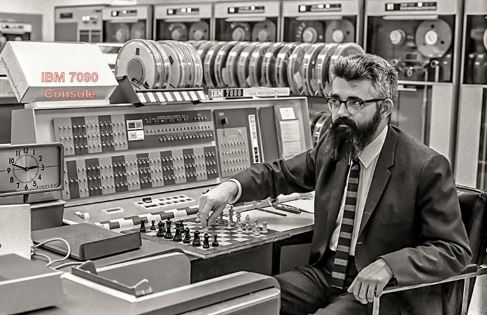
\includegraphics[scale=0.5]{figures/contoh.JPG}
\caption{capturing}
\label{contoh}
\end{figure}

\par Jika kita berbicara tentang AI atau Artificial Intelligence maka kita tidak bisa melupakan seorang sosok yang sangat terkenal pada bidang tersebut yaitu bapak John McCarthy.
McCarthy mendapatkan gelar sarjana matematika dari California Institute of Technology (Caltech) pada September 1948. Dari masa kuliahnya itulah ia mulai mengembangkan ketertarikannya pada mesin yang dapat menirukan cara berpikir manusia. McCarthy kemudian melanjutkan pendidikan ke program doktoral di Princeton University.

\par McCarthy kemudian mendirikan dua lembaga penelitian kecerdasan buatan. Kedua lembaga AI itu adalah Stanford Artificial Intelligence Laboratory dan MIT Artificial Inteligence Laboratory. Di lembaga-lembaga inilah bermunculan inovasi pengembangan AI yang meliputi bidang human skill, vision, listening, reasoning dan movement of limbs. Bahkan Salah satu lembaga yang didirikan itu, Stanford Artificial Intelligence pernah mendapat bantuan dana dari Pentagon untuk membuat teknologi-teknologi luar angkasa.

\item Perkembangan Kecerdasan Buatan
\par Teknologi Artificial Intelligence semakin ramai dibahas dalam berbagai diskusi teknologi di seluruh dunia.Menurut kebanyakan orang, pekerjaan seperti kasir, operator telepon, pengendara truk, dan lainnya sangat berpeluang besar untuk tergantikan oleh Artificial Intelligence. Mengapa terjadi hal demikian? dikarenakan memang bahwa AI lebih ungul dalam hal kinerja, fitur dan lain sebagainya. Namun, dalam beberapa aspek memang pekerja manusia masih unggul dibandingkan AI itu sendiri.
\par Para generasi muda yang ada di dunia terutama di daerah Asia terlihat sudah memahami fungsi dan efek dari AI dalam kehidupan kita sehari-hari. Berdasarkan survei yang dilakukan oleh Microsoft, terdapat 39 persen responden yang mempertimbangkan untuk menggunakan mobil tanpa pengemudi dan 36 persen lainnya setuju bahwa robot masa depan dengan software untuk beroperasi mampu meningkatkan produktivitas. Dari survey tersebut kita sebagai pengguna AI harus lebih bijaksana dalam pengembangan dan penggunaan dari AI sehingga tanpa memberikan efek samping terhadap etos kerja dan keseharian kita sebagai pengguna dalam kehidupan sehari-hari.
\end{itemize}
\item Tentang Pengertian Terhadap Ilmu Yang Lain
\begin{itemize}
\item Supervised Learning adalah pendekatan dimana sudah terdapat data yang dilatih selain itu juga terdapat variable yang ditargetkan sehingga tujuan dari pendekatan ini yaitu mengkelompokan suatu data ke data yang sudah ada.
\par
\item Klasifikasi adalah pembagian sesuatu menurut kelas-kelas ( class ). Menurut Ilmu Pengetahuan, Klasifikasi merupakan proses pengelompokkan benda berdasarkan ciri-ciri persamaan dan juga perbedaan.
\par
\item Regresi adalah metode analisis statistik yang digunakan untuk melihat pengaruh antara dua ataupun lebih variabel.
\par
\item Unsupervised Learning berbeda dengan Supervised Leraning. Perbedaannya ialah unsupervised learning tidak memiliki data latih, sehingga dari data yang ada kita mengelompokan data tersebut menjadi 2  ataupun 3 bagian dan seterusnya.
\par
\item Dataset adalah objek yang merepresentasikan data dan juga relasi yang ada di memory. Strukturnya mirip dengan data di database, namun bedanya dataset berisi koleksi dari data table dan data relation.
\par
\item Training Set adalah set digunakan oleh algoritma klassifikasi . Dapat dicontohkan dengan :  decision tree, bayesian, neural network dll. Semuanya dapat digunakan untuk membentuk sebuah model classifier.
\par
\item Testing Set adalah set yang digunakan untuk mengukur sejauh mana classifier berhasil melakukan klasifikasi dengan benar.
\par
\end{itemize}
\end{enumerate}


\subsection{Instalasi}
Untuk Instalasinya mencakup i beberapa pembahasan dan tutorial. yaitu :
\begin{enumerate}
\item Instalasi Scikit-Learn Dari Anaconda
\begin{itemize}
\item Instalasi Anaconda
\begin{enumerate}
\item Pertama-tama silahkan pastikan bahwa anda telah melakukan instalasi software Anaconda.
\item Apabila belum, silahkan buka web browser anda untuk melakukan pengunduhan software Anaconda
\item Setelah terunduh, silahkan klik kanan lalu run administrator pada software Anaconda
\item Silahkan lakukan penginstalan dengan menekan tombol install pada tampilan instalasi
\item Kemudian tekan tombol next maka akan sampai pada tampilan diatas

\par

\begin{figure}[ht]
\centering
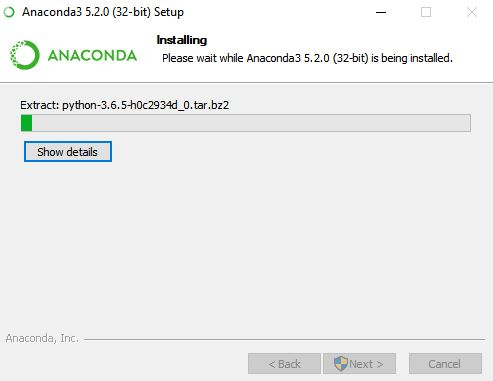
\includegraphics[scale=0.5]{figures/ana1.JPG}
\caption{install anaconda 1}
\label{contoh}
\end{figure}

\par
\item Selanjutnya apabila instalan tersebut telah selesai maka silahkan menekan tombol next
\item Tampilan selanjutnya akan seperti ini

\par

\begin{figure}[ht]
\centering
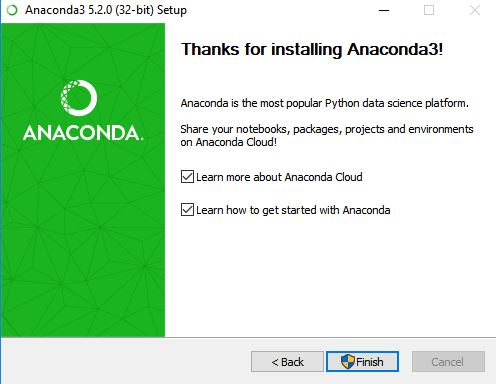
\includegraphics[scale=0.5]{figures/ana2.JPG}
\caption{install anaconda 2}
\label{contoh}
\end{figure}

\par

\item Apabila tampilannya telah sesuai dengan contoh gambar maka instalasi telah selesai
\end{enumerate}
\end{itemize}

\begin{itemize}
\item Instalasi Library Scikit Learn
\begin{enumerate}
\item Silahkan membuka web browser untuk melakukan pengunduhan untuk library scikit dari anaconda.
\item Silahkan mengunjungi halaman ini untuk melakukan pengunduhan library scikit dari anaconda.
\par https://anaconda.org/anaconda/scikit-learn.
\item Setelah terdownload silahkan melakukan instalasi lanjutan menggunakan Command Prompt
\item Silahkan masukkan perintah berikut untuk melakukan pengecekan bahwa anaconda anda telah terpasang dengan baik.
\par conda --version
\par python --version
\item Tampilannya akan nampak seperti berikut :
\par

\begin{figure}[ht]
\centering
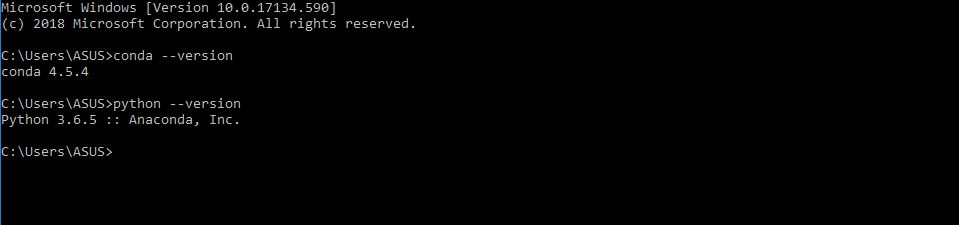
\includegraphics[scale=0.3]{figures/scikit1.JPG}
\caption{Pengecekan Anaconda}
\label{contoh}
\end{figure}

\par
\item Selanjutnya silahkan masukkan perintah berikut untuk melakukan instalasi pip sckit-learn
\par perintahnya : pip install -U scikit-learn
\item Tampilannya akan nampak seperti berikut :
\par

\begin{figure}[ht]
\centering
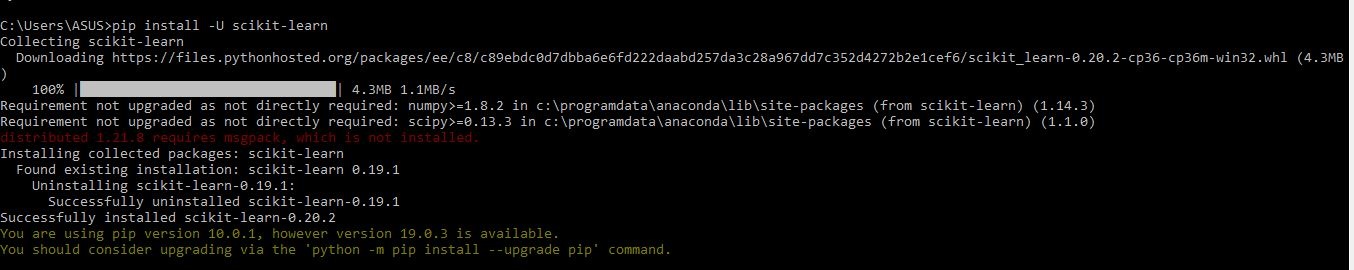
\includegraphics[scale=0.2]{figures/scikit3.jpg}
\caption{instalasi pip scikit-learn}
\label{contoh}
\end{figure}

\par
\item Selanjutnya silahkan masukkan perintah berikut untuk melakukan instalasi conda sckit-learn
\par perintahnya : conda install scikit-learn
\item Tampilannya akan nampak seperti berikut :
\par

\begin{figure}[ht]
\centering
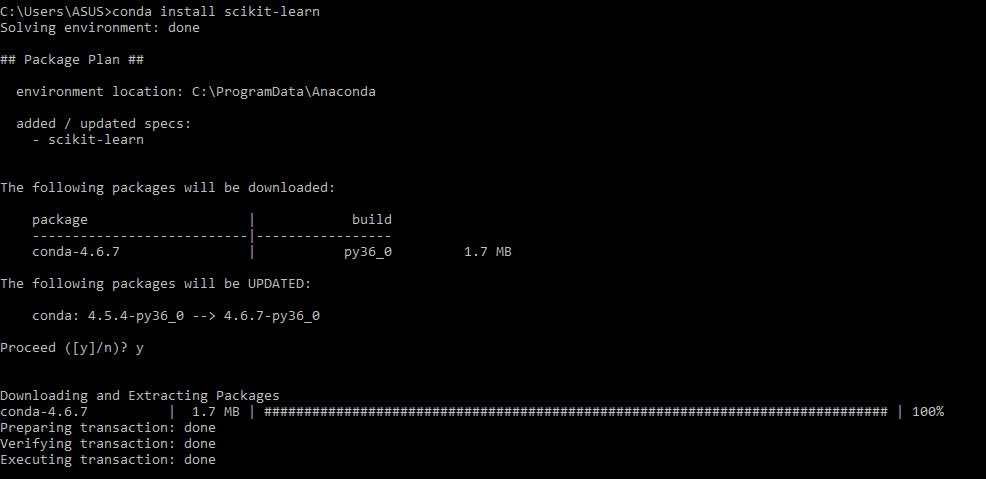
\includegraphics[scale=0.3]{figures/scikit4.JPG}
\caption{instalasi conda scikit-learn}
\label{contoh}
\end{figure}

\par
\par
\par
\item Apabila telah dipraktekan seperti langkah-langkah dan menghasilkan tampilan seperti contoh diatas, maka instalasi scikit-learn dari anaconda berhasil dilakukan
\par
\item Kemudian untuk pengujian yang lain yaitu pengujian untuk mengecek codingan anaconda
\par
\item Contoh uji coba codingannya dapat dilihat pada gambar berikut
\par
\begin{figure}[ht]
\centering
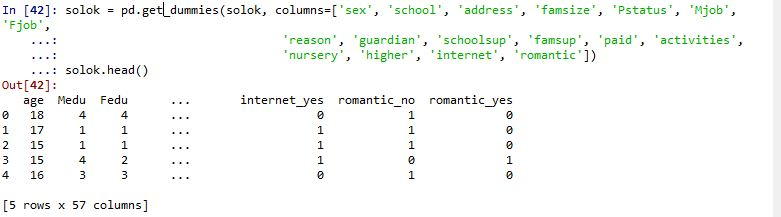
\includegraphics[scale=0.5]{figures/3.JPG}
\caption{uji coba codingan}
\label{contoh}
\end{figure}
\par
\item Berdasarkan pengujian tersebut maka dapat dipastikan bahwa anaconda telah ter-include ke dalam python dan dieksekusi dengan script python
\item Setelah pengeksekusiannya berdasarkan scripts python, terdapatlah keluaran yang sesuai
\item Keluaran tersebut yang menandakan bahwa anacondanya berfungsi dengan baik.
\end{enumerate}
\end{itemize}


\par
\item Loading An Example Dataset
\begin{itemize}
\item Penerapan Loading An Example Dataset Pada Python Di CMD
\begin{enumerate}
\item Pertama-tama silahkan buka command prompt di laptop anda
\item Selanjutnya masuk ke python
\item Setelah masuk kedalam python, silahkan masukkan perintah seperti pada gambar berikut :

\begin{figure}[ht]
\centering
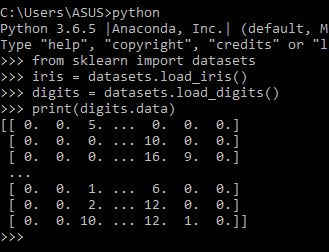
\includegraphics[scale=0.6]{figures/4.JPG}
\caption{pengujian loading an example dataset}
\label{contoh}
\end{figure}

\par
\item Secara keseluruhan, hasilnya pada command prompt akan nampak seperti gambar tersebut
\item Apabila tampilanya telah nampak seperti gambar diatas, maka pengujiannya telah selesai dan berhasil.
\end{enumerate}

\par
\item Penjelasan Perintah Yang Di Uji
\begin{enumerate}
\item Perhatikan perintah yang telah dieksekusi ini :

\par
\begin{figure}[ht]
\centering
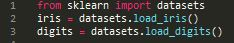
\includegraphics[scale=0.9]{figures/ok4.JPG}
\caption{pengujian loading an example dataset}
\label{contoh}
\end{figure}
\par

\item Penjelasan untuk baris pertama ialah :
\par Perintahnya yaitu memasukkan dan memanggil dataset dari sklearn
\par
\par
\item Penjelasan untuk baris kedua ialah :
\par Terdapat variabel baru yaitu iris. Dimana variabel iris memanggil datasets dan di dalamnya akan ngeload ( menampilkan ) load iris.
\par
\item Penjelasan untuk baris ketiga ialah :
\par Kemudian ada juga variabel baru lainnya yaitu digits yang akan memanggil dataset dan di dalamnya akan ngeload ( menampilkan ) load digits
\par
\item Selanjutnya untuk perintah Print( digits.data ) ditujukan untuk me-
\par nampilkan output dari pengeksekusian variabel digits dan akan berupa data.
\par
\item Hasilnya printnya sebagai berikut :
\par

\begin{figure}[ht]
\centering
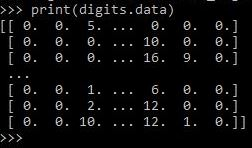
\includegraphics[scale=0.7]{figures/okk4.JPG}
\caption{hasil print uji cobat}
\label{contoh}
\end{figure}

\par
\item Untuk penjelasan uji cobanya sudah selesai.
\par
\end{enumerate}
\end{itemize}
\end{enumerate}

\section{Rahmi Roza/1164085}
\subsection{Teori}
Teori mencakup resume dari beberapa pembahasan. yaitu :
\begin{itemize}
\item Definisi Kecerdasan Buatan.
\par Kecerdasan Buatan adalah salah satu cabang Ilmu pengetahuan berhubungan dengan pemanfaatan mesin untuk memecahkan persoalan yang rumit dengan cara yang lebih manusiawi. Hal Ini biasanya dilakukan dengan mengikuti/mencontoh karakteristik dan analogi berpikir dari kecerdasan/Inteligensia manusia, dan menerapkannya sebagai algoritma yang dikenal oleh komputer.
\par Agar komputer bisa bertindak seperti dan sebaik manusia, maka komputer juga harus diberi bekal pengetahuan dan mempunyai kemampuan untuk menalar. Untuk itu AI akan mencoba untuk memberikan beberapa metoda untuk membekali komputer dengan kedua komponen tersebut agar komputer bisa menjadi mesin pintar.
\item Sejarah Kecerdasan Buatan
\par Banyak orang percaya kecerdasan buatan akan memusnahkan kelangsungan hidup manusia saat mereka menyadari kekuatan yang dimilikinya. Semua bermula sejak Turing Machine. Berikut perjalanan kecerdasan buatan hingga akhirnya melahirkan robot dan robot seks.
\par Tahun 1950. Alan Turing memperkenalkan Turing Test dalam jurnal berjudul Computering Machinery and Intelligence. Pada musim panas 1956, Konferensi Dartmouth meluncurkan ide artificial intelligence dan IBM memulai riset tentang AI.
\par Tahun 1970. Sepanjang 1974 sampai 1980 merupakan gelombang pertama kecerdasan buatan. Pada periode ini pula pengumpulan dana untuk melakukan riset kecerdasan buatan mulai marak.
\par Tahun 1930. Pada 11 Mei 1997, Deep Blue Computer, kecerdasan buatan besutan IBM berhasil mengalahkan grand master catur asal Rusia, Garry Kasparov
\par Tahun 2000. Kendaraan bikinan tim peneliti dari Universitas Stanford, Amerika Serikat, berhasil menjadi kampiun dal DARPA Grand Challange. Mobil swakemudi ini bisa melaju di gurun pasir sejauh 211 kilometer.
\par Tahun 2010. Watson, kecerdasan buatan besutan IBM, berhasil mengalahkan mantan juara Brad Rutter dan Ken Jennings dalam acara kuis Jeopardy pada pertengahan 2011. Appel, pada 14 Oktober tahun yang sama, memperkenalkan asistem pribadi berbasiskan kecerdasan buatan bernama Siri dalam iPhone 4s. Setahun kemudian, tepatnya Juni, tim dari Google Brain melatih komputer agar bisa mengenali seekor kucing dari jutaan video di YouTube.ChatBot bikinin Eugene Goostman mengklaim telah memecahkan tes Turing dalam kompetisi yang digelar di Universitas Reading, Inggris. Imbasnya, pada Agustus tahun yang sama, banyak ilmuwan mengusulkan untuk membuat tes Turing yang baru. Sementara itu, terkesan dengan kemampuan Watson, NASA menggunakannya untuk penelitian bidang kedirgantaraan.
\par Tahun 2017. Google, Februari lalu, kembali membuat gebrakan soal kecerdasan buatan. Tim dari Google Deep Mind mengungkap kecerdasan buatan memiliki tingkat emosi dan kemarahan yang sama dengan manusia. Kecerdasan buatan pun bisa merasakan kalau dirinya ditipu. Tak mau kalah, Microsoft, April lalu, mendeteksi bahwa artificial intelligence ternyata juga bisa rasis.
Yang paling fenomenal soal kecerdasan buatan pada tahun ini adalah robot seks bernama Harmony. Tak seperti robot seks pada umumnya, Harmony bisa merasakan cemburu dan mendeteksi penggunanya saat hendak menuju klimaks.
\par Jika kita berbicara tentang AI atau Artificial Intelligence maka kita tidak bisa melupakan seorang sosok yang sangat terkenal pada bidang tersebut yaitu bapak John McCarthy.
McCarthy mendapatkan gelar sarjana matematika dari California Institute of Technology (Caltech) pada September 1948. Dari masa kuliahnya itulah ia mulai mengembangkan ketertarikannya pada mesin yang dapat menirukan cara berpikir manusia. McCarthy kemudian melanjutkan pendidikan ke program doktoral di Princeton University.
\par McCarthy kemudian mendirikan dua lembaga penelitian kecerdasan buatan. Kedua lembaga AI itu adalah Stanford Artificial Intelligence Laboratory dan MIT Artificial Inteligence Laboratory. Di lembaga-lembaga inilah bermunculan inovasi pengembangan AI yang meliputi bidang human skill, vision, listening, reasoning dan movement of limbs. Bahkan Salah satu lembaga yang didirikan itu, Stanford Artificial Intelligence pernah mendapat bantuan dana dari Pentagon untuk membuat teknologi-teknologi luar angkasa.

\item Perkembangan Kecerdasan Buatan
\par Perkembangan kecerdasan buatan atau artificial intelligence (AI) dinilai tidak bisa dihentikan. Keberadaan AI justru dinilai akan semakin mempermudah kehidupan manusia dalam beraktivitas. Dalam pandangan Johnny Lie sebagai Vice President of Cheetah Mobile, revolusi teknologi tidak bisa dihentikan. Menurutnya, hal itu sudah terjadi sejak puluhan tahun yang lalu. Cheetah Mobile sendiri merupakan perusahaan teknologi mobile yang fokus pada peranti lunak dan pada hari ini menyematkan unsur AI dalam layanannya.
\par Sebelumnya, beberapa pakar teknologi kenamaan dunia, seperti Elon Musk dan Stephen Hawking gencar memberikan peringatan bahwa AI yamg terus berkembang dapat menjadi ancaman bagi umat manusia. Bahkan, keduanya bersama banyak ilmuwan lainnya membuat surat penegasan kepada PBB untuk mengawasi pertumbuhan AI.
\par Dengan AI, sebuah produk teknologi dapat bekerja lebih cerdas dan mandiri. Misalnya saja, sebuah aplikasi smartphone yang menggunakan AI dapat mempelajari kebiasaan pengguna. Alhasil, Anda tidak perlu repot lagi dalam melakukan suatu pekerjaan di ponsel.
\end{itemize}
\item Tentang Pengertian Terhadap Ilmu Yang Lain
\begin{itemize}
\item Supervised learning adalah sebuah pendekatan dimana sudah terdapat data yang dilatih, dan terdapat variable yang ditargetkan sehingga tujuan dari pendekatan ini adalah mengkelompokan suatu data ke data yang sudah ada
\par
\item Klasifikasi adalah pembagian sesuatu menurut kelas-kelas ( class ). Menurut Ilmu Pengetahuan, Klasifikasi merupakan proses pengelompokkan benda berdasarkan ciri-ciri persamaan dan juga perbedaan.
\par
\item Regresi adalah metode analisis statistik yang digunakan untuk melihat pengaruh antara dua ataupun lebih variabel.
\par
\item Unsupervised Learning berbeda dengan Supervised Leraning. Perbedaannya ialah unsupervised learning tidak memiliki data latih, sehingga dari data yang ada kita mengelompokan data tersebut menjadi 2  ataupun 3 bagian dan seterusnya.
\par
\item Dataset adalah objek yang merepresentasikan data dan juga relasi yang ada di memory.
\par
\item Training Set adalah set digunakan oleh algoritma klassifikasi . Dapat dicontohkan dengan :  decision tree, bayesian, neural network dll. Semuanya dapat digunakan untuk membentuk sebuah model classifier.
\par
\item Testing Set adalah set yang digunakan untuk mengukur sejauh mana classifier berhasil melakukan klasifikasi dengan benar.
\par
\end{itemize}
\end{enumerate}

\subsection{Instalasi}
\begin{figure}[ht]
\centering
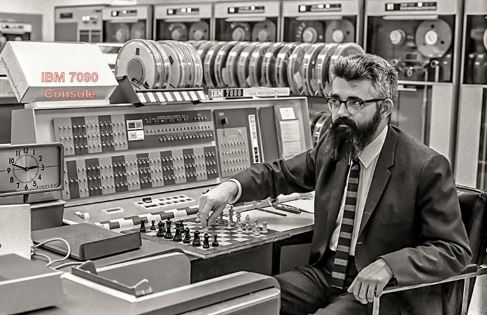
\includegraphics[scale=0.5]{figures/contoh.jpg}
\caption{gambar1}
\label{roza1}
\end{figure}

\begin {enumerate}
\item Baris 1 = memasukkan dan memanggil svm dari sklearn
\item Baris 2 = membuat variable
\end {enumerate}

\begin{figure}[ht]
\centering
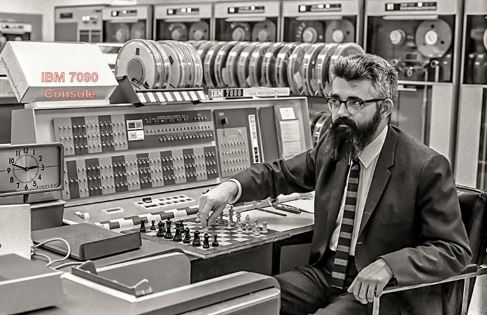
\includegraphics[scale=0.7]{figures/contoh.jpg}
\caption{gambar2}
\label{roza2}
\end{figure}

\begin {enumerate}
\item Baris 1 = clf dipasang pada model fit metode
\item Baris 2 =  implementasikan klasifikasi dukungan vektor
\end {enumerate}

\begin{figure}[ht]
\centering
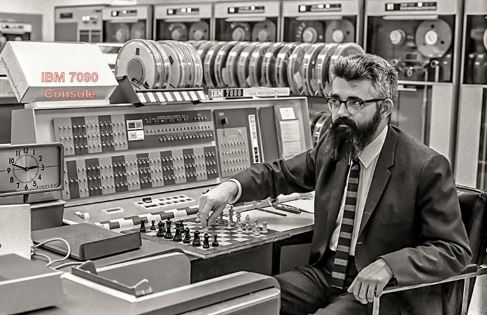
\includegraphics[scale=0.5]{figures/contoh.jpg}
\caption{gambar3}
\label{roza3}
\end{figure}

\begin {enumerate}
\item Baris 1 = prediksi nilai baru
\item Baris 2 = set array
\end {enumerate}

\begin{figure}[ht]
\centering
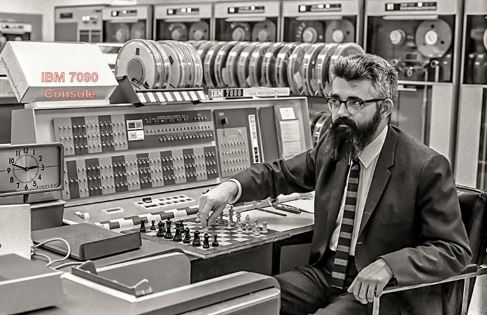
\includegraphics[scale=0.10]{figures/contoh.jpg}
\caption{gambar4}
\label{roza4}
\end{figure}

\begin {enumerate}
\item Baris 1 = memasukkan dan memanggil datasets dari sklearn
\item Baris 2 = memasukkan dan memanggil svm dari sklearn
\item Baris 3 = membuat variable clf
\item Baris 4 = membuat variable iris
\item Baris 5 = membuat variable x, y
\item Baris 6 = clf dipasang pada model fit metode
\item Baris 7 = implementasikan klasifikasi dukungan vektor
\item Baris 8 = memanggil library pickle
\item Baris 9 = membuat variable s
\item Baris 10 = membuat variable clf2
\item Baris 11 = prediksi nilai baru
\item Baris 12 = set array
\end {enumerate}

\begin{figure}[ht]
\centering
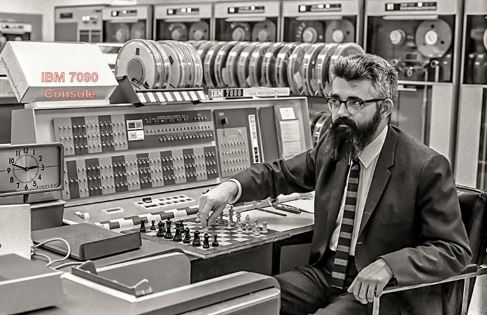
\includegraphics[scale=0.7]{figures/contoh.jpg}
\caption{gambar5}
\label{roza5}
\end{figure}

\begin {enumerate}
\item Baris 1 = memasukkan dan memanggil numpy sebagai np
\item Baris 2 = memasukkan dan memanggil random_projection dari sklearn
\item Baris 3 = membuat variable rng
\item Baris 4 = membuat variable rng
\item Baris 5 = membuat variable x
\item Baris 6 = pemanggilan variable x
\item Baris 7 = pemanggilan dtype
\item Baris 8 = membuat variable tranformer
\item Baris 9 = membuat variable x_new
\item Baris 10 = pemanggilan x_new
\item Baris 11 = pemanggilan dtype
\end {enumerate}

\subsection{Penanganan Error}
\item Skrinsut Error.
\begin{figure}[ht]
\centering
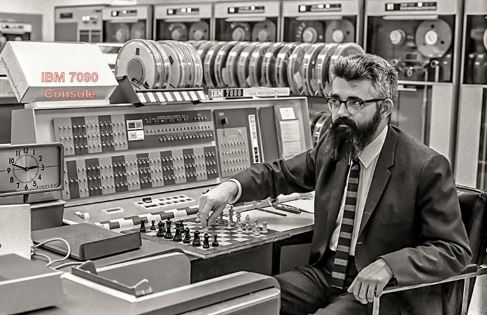
\includegraphics[scale=0.7]{figures/contoh.jpg}
\caption{gambar6}
\label{roza6}
\end{figure}
\item Tuliskan kode eror dan jenis errornya
\begin{itemize}
\item Kode error = NameError: name 'roza' is not defined
\item jenis error = NameError
\end{itemize}
\item  Solusi pemecahan masalah error
\begin{figure}[ht]
\centering
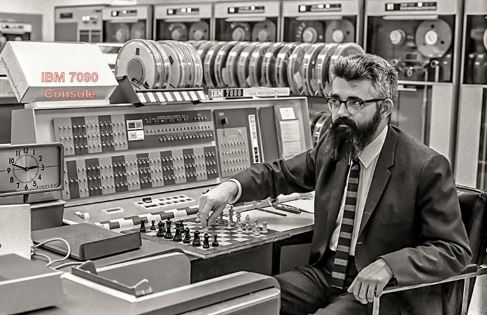
\includegraphics[scale=0.7]{figures/contoh.jpg}
\caption{gambar7}
\label{roza7}
\end{figure}



\section{Lusia Violita Aprilian/1164080}
\subsection{Artificial Intelegence}
\begin{enumerate}
	\item Pengertian AI\\
	Menurut Minsky, Kecerdasan Buatan ialah suatu ilmu yang mempelajari cara membuat 			komputer melakukan sesuatu seperti yang dilakukan oleh manusia. Lalu menurut Ensiklopedi Britannica, Kecerdasan Buatan ialah cabang ilmu komputer yang merepresentasi pengetahuan lebih banyak menggunakan symbol-simbol daripada bilangan, dan memproses informasi berdasarkan metode heuristic atau berdasarkan jumlah aturan.

	Menurut Stuart J. Russell & Peter Norvig, Kecerdasan Buatan ialah perangkat komputer yang dapat memahami lingkungannya dan dapat mengambil tindakan yang memaksimalkan peluang kesuksesan di lingkungan tersebut untuk beberapa tujuan.

Berdasarkan beberapa teori tentang kecerdasan buatan diatas, penulis menyimpulkan bahwa kecerdasan buatan adalah suatu ilmu yang membuat sebuah mesin menjadi cerdas, sehingga kecerdasan mesin tersebut mirip dengan kecerdasan manusia serta dapat mengambil keputusan sendiri untuk menyelesaikan sebuah masalah.

	\item Sejarah dan Perkembangan
	\begin{itemize}
		\item 1941 ( Era Komputer Elektronik )\\
    Pada era ini, telah ditemukan pertama kali yakni alat penyimpanan dan pemrosesan informasi atau disebut komputer elektronik. Ini juga digunakan untuk dasar pengembangan program ke arah AI.
    \item 1943 – 1956 ( Era Persiapan AI )\\
    Pada tahun 1943, terdapat dua peneliti yakni Warren McCulloch dan Walter Pitts yang berhasil membuat sebuah model tiruan dari tiap neuron seperti on dan off. Mereka membuktikan bahwa setiap fungsi dapat dihitung dengan suatu jaringan sel saraf dan semua hubungan logis bisa diimplementasikan dengan struktur jaringan yang sederhana.\\
    Pada tahun 1950, Norbert Wiener melakukan penelitian tentang prinsip teori feedback. Bentuk implementasi dari penelitian tersebut salah satunya adalah thermostat.\\
    Pada tahun 1956, John McCarthy mencoba meyakinkan Minsky, Claude Shannon, dan Nathaniel Rochester untuk membantunya dalam melakukan penelitian di bidang automata, jaringan saraf, dan pembelajaran intelijensia. Mereka mengerjakan proyek ini kurang lebih selama 2 bulan di Universitas Dartmouth. Hasilnya adalah berupa program yang mampu berpikir non-numerik dan menyelesaikan masalah pemikiran, yang disebut Principia Mathematica. Berdasarkan hal ini, telah ditentukan bahwa McCarthy disebut sebagai father of Artificial Intelligence/ Bapak Kecerdasan Buatan.
    \item 1952 – 1969 ( Awal Perkembangan )\\
    Pada tahun 1958, McCarthy di MIT AI Lab mengeluarkan bahasa pemrograman tingkat tinggi yaitu LISP, dimana sekarang sudah mulai sering digunakan dalam pembuatan program-program AI. Lalu, McCarthy membuat program yang disebut programs with common sense. Di program tersebut, dibuat sebuah rancangan untuk menggunakan pengetahuan dalam mencari solusi dari sebuah masalah.\\
    Pada tahun 1959, Program komputer bernama General Problem Solver berhasil dibuat oleh Herbert A. Simon, J.C. Shaw, dan Allen Newell. Program tersebut dirancang untuk memulai proses penyelesaian masalah secara manusiawi. Pada tahun yg sama Nathaniel Rochester dari IBM dan para mahasiswanya merilis sebuah program AI yaitu geometry theorem prover. Program ini dapat mebuktikan bahwa suatu teorema menggunakan axioma-axioma yang ada.\\
    Pada tahun 1963, program yang dibuat oleh James Slagle bisa menyelesaikan masalah integral tertutup untuk mata kuliah Kalkulus.\\
    Pada tahun 1968, program analogi buatan Tom Evan dapat menyelesaikan masalah analogi geometri yang ada pada tes IQ.
    \item 1966 – 1974 ( Perkembangan AI Lambat )\\
    Perkembangan AI mulai melambat pada tahun 1966 – 1974, yang disebabkan adanya beberapa kesulitan yang di hadapi seperti  Program-program AI yang bermunculan hanya mengandung sedikit atau bahkan tidak mengandung sama sekali pengetahuan pada subjeknya, banyak terjadi kegagalan pada pembuatan program AI, serta terdapat beberapa batasan pada struktur dasar yang digunakan untuk menghasilkan perilaku intelijensia.
    \item 1969 – 1979 (Sistem berbasis pengetahuan )\\
    Pada tahun 1960, Ed Feigenbaum, Bruce Buchanan, dan Joshua Lederberg mulai merintis proyek bernama DENDRAL yaitu program yang digunakan untuk memecahkan masalah struktur molekul dari informasi yang didapatkan dari spectometer massa. Dari segi diagnosa medis juga terdapat  yang menemukan sistem berbasis Ilmu pengetahuan, yaitu Saul Amarel dalam proyek computer ini biomedicine. Proyek ini diawali dari keinginan untuk mendapatkan diagnosa penyakit berdasarkan pengetahuan yang ada pada mekanisme penyebab proses penyakit.
    \item 1980 – 1988 ( AI menjadi Industri )\\
    Industralisasi AI diawali dengan ditemukannya sebuah sistem pakar yang dinamakan R1 yang mampu mengkonfigurasi sistem-sistem komputer baru. Program tersebut mulai dijalankan di Digital Equipment Corporation (DEC), McDermott, pada tahun 1982. Pada tahun 1986, program ini telah berhasil menghemat biaya sebesar US 40 juta per tahun.\\
    Pada tahun 1988, kelompok AI di DEC menjalankan program sistem pakar sebanyak 40 sistem pakar. Hampir semua perusahaan besar di USA mempunyai divisi Ai sendiri yang menggunakan maupun mempelajari sistem pakar itu sendiri. Industri AI yang sedang ramai diperbincangkan juga melibatkan perusahaan-perusahaan besar seperti Carnegie Group, Inference, IntelliCorp, dan Technoledge yang menawarkan software tools untuk membangun sistem pakar. Perusahaan bidang hardware seperti LISP Machines Inc., Texas Instruments, Symbolics, dan Xerox dan lain-lain juga ikut berperan dalam membangun sebuah workstation yang dioptimasi untuk pembangunan program LISP. Sehingga, perusahaan yang sudah berdiri sejak tahun 1982 hanya menghasilkan beberapa juta US dollar per tahun meningkat menjadi 2 milyar US dollar per tahun pada tahun 1988.
    \item 1986 – sekarang ( kembalinya jaringan saraf tiruan )
    Meskipun bidang ilmu komputer, telah melakukan penolakan terhadap jaringan saraf tiruan setelah diterbitkannya sebuah buku berjudul ‘Perceptrons’ karangan Minsky dan Papert, tetapi para ilmuwan masih terus mempelajari bidang ilmu tersebut dari sudut pandang yang lain, yaitu bidang fisika. Ahli fisika seperti Hopfield (1982) menggunakan teknik-teknik mekanika statistika untuk menganalisa sifat-sifat penyimpanan dan optimasi pada jaringan saraf. ahli psikolog, David Rumhelhart dan Geoff Hinton melanjutkan penelitian tersebut tentang model jaringan saraf pada memori. Pada tahun 1985-an sedikitnya empat kelompok riset menemukan algoritma Back-Propagation. Algoritma inipun akhirnya berhasil diimplementasikan ke dalam ilmu bidang komputer dan psikologi.
	\end{itemize}		
\end{enumerate}

\subsection{Supervised Learning dan Data}
\begin{enumerate}
	\item Supervised Learning\\
	Sebuah pendekatan dengan kondisi dimana sudah ada terdapat kumpulan data yang dilatih atau ditraining, dan terdapat beberapa variabel yang sudah ditentukan sehingga tujuan dari pendekatan tersebut mengarah ke data yang sudah ada.
	
	\item Klasifikasi\\
	Sebuah sejenis program yang dapat menentukan objek yang ada termasuk jenis apa berdasarkan variabel-variabel yang sudah ditentukan.
	
	\item Regresi\\
	Sebuah metode yang digunakan untuk menentukan dan memprediksi berdasarkan hubungan sebab – akibat antara satu variabel ke variabel lainnya.
	
	\item Unsupervised Learning\\
	Sebuah pendekatan yang dimana tidak memiliki data yang dilatih, namun ingin di kelompokkan berdasarkan beberapa variabel dengan kemauan sendiri.
	
	\item Data Set\\
	Objek yang merepresentasikan data dan relasi didalam memori.

	\item Training Set\\
	Himpunan dari berbagai pasangan objek, kelas yang dapat menunjukkan objek tersebut yang sudah diberi label.

	\item Testing Set\\
	Himpunan data yang sudah berlabel lain, yang digunakan untuk mengukur persentase sampel yang diklasifikan dengan benar atau persentase sampel mengalami kesalahan.

\end{enumerate}

\subsection{Learning and Predicting}
\begin{enumerate}
	\item Learning and predicting 1
			\begin{figure}[ht]
			\centering
			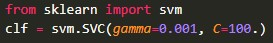
\includegraphics[scale=0.5]{figures/b1.jpg}
			\caption{Learning and predicting 1}
			\label{contoh}
			\end{figure}
			\begin{itemize}
			    \item Baris 1 = memasukkan dan memanggil svm dari sklearn
			    \item Baris 2 = membuat variable
			\end{itemize}

	\item Learning and predicting 2
		\begin{figure}[ht]
		\centering
		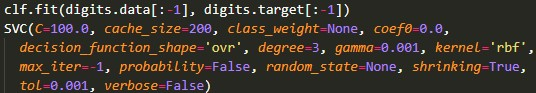
\includegraphics[scale=0.5]{figures/b2.jpg}
		\caption{Learning and predicting 2}
		\label{contoh}
		\end{figure}
		\begin{itemize}
			    \item Baris 1 = clf dipasang pada model fit metode
			    \item Baris 2 =  implementasikan klasifikasi dukungan vektor
			\end{itemize}
			
	\item Learning and predicting 3
		\begin{figure}[ht]
		\centering
		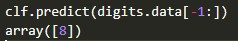
\includegraphics[scale=0.5]{figures/b3.jpg}
		\caption{Learning and predicting 3}
		\label{contoh}
		\end{figure}
		\begin{itemize}
			    \item Baris 1 = prediksi nilai baru
			    \item Baris 2 = set array
			\end{itemize}
\end{enumerate}

\subsection{Model Persistence}
\begin{enumerate}
	\item menjelaskan maksud dari tulisan tersebut dan mengartikan per baris.
		\begin{figure}[ht]
		\centering
		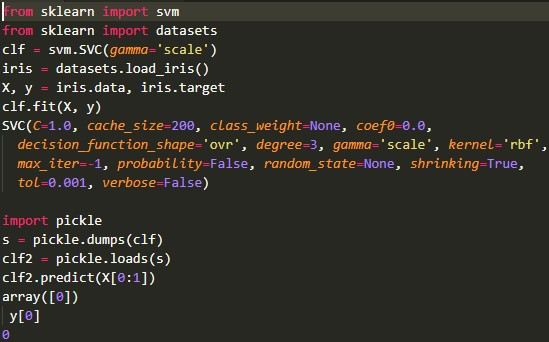
\includegraphics[scale=0.5]{figures/c1.jpg}
		\caption{Model Persistence}
		\label{contoh}
		\end{figure}
	\begin{itemize}
			   \item Baris 1 = memasukkan dan memanggil datasets dari sklearn
                \item Baris 2 = memasukkan dan memanggil svm dari sklearn
                \item Baris 3 = membuat variable clf
               \item Baris 4 = membuat variable iris
               \item Baris 5 = membuat variable x, y
               \item Baris 6 = clf dipasang pada model fit metode
               \item Baris 7 = implementasikan klasifikasi dukungan vektor
               \item Baris 8 = memanggil library pickle
               \item Baris 9 = membuat variable s
              \item  Baris 10 = membuat variable clf2
               \item Baris 11 = prediksi nilai baru
              \item  Baris 12 = set array

			\end{itemize}
\end{enumerate}

\subsection{Conventions}
\begin{enumerate}
	\item menjelaskan maksud dari tulisan tersebut dan mengartikan per baris.
		\begin{figure}[ht]
		\centering
		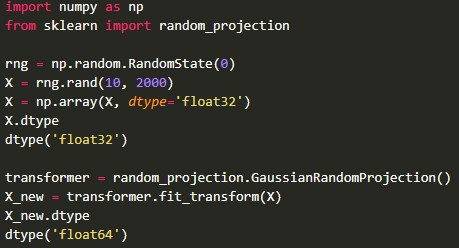
\includegraphics[scale=0.5]{figures/d1.jpg}
		\caption{Conventions}
		\label{contoh}
		\end{figure}
		\begin{itemize}
			 \item   Baris 1 = memasukkan dan memanggil numpy sebagai np
             \item   Baris 2 = memasukkan dan memanggil random projection dari sklearn
             \item   Baris 3 = membuat variable rng
             \item   Baris 4 = membuat variable rng
             \item   Baris 5 = membuat variable x
             \item   Baris 6 = pemanggilan variable x
             \item   Baris 7 = pemanggilan dtype
             \item   Baris 8 = membuat variable tranformer
             \item   Baris 9 = membuat variable xnew
             \item   Baris 10 = pemanggilan xnew
             \item   Baris 11 = pemanggilan dtype

			\end{itemize}
\end{enumerate}

\subsection{Penanganan Error}
Dari percobaan yang dilakukan di atas, apabila mendapatkan error maka:

\begin{enumerate}
	\item skrinsut error
		\begin{figure}[ht]
		\centering
		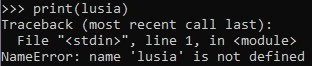
\includegraphics[scale=0.5]{figures/e1.jpg}
		\caption{skrinsut error}
		\label{contoh}
		\end{figure}
	\item Tuliskan kode eror dan jenis errornya
	\begin{itemize}
			    \item Kode error = NameError: name 'lusia' is not defined
			    \item jenis error = NameError
			\end{itemize}

	\item  Solusi pemecahan masalah error
		\begin{figure}[ht]
		\centering
		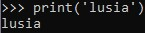
\includegraphics[scale=0.5]{figures/e2.jpg}
		\caption{gb 1}
		\label{contoh}
		\end{figure}

\end{enumerate}

